%% ======================================================================
%%  PPoPP Paper Template (ACM SIGPLAN, acmart sigplan, 10pt, two-column)
%%  Based on acmart v2.20 (2026/08/16)
%%
%%  使用方式請見 README.md
%%  PPoPP 規範重點：
%%    * acmart + sigplan 選項 + 10pt 字級（雙欄）
%%    * 正文（含圖表）最多 10 頁，參考文獻不計頁數、不限長度
%%    * 雙盲審查：不得出現作者姓名、單位；引用自己的研究請用第三人稱
%%    * 不可附 appendix（補充資料另以 PDF/ZIP 上傳）
%%    * 不可調整版面（vspace、邊界、行距、欄距等）
%%    * 圖說（caption）字級 >= 9pt；圖表內文字 >= 8pt
%%    * 參考文獻需列出所有作者（不可 et al.）、年份與出版處
%% ======================================================================

%% ---------------- 模式切換：只需改這一行 ----------------
%%   true  = 投稿版（匿名、無行號、有頁碼、不印 CCS/ACM Reference）
%%   false = Camera-ready 最終版（錄取後使用）
\newif\ifsubmission
\submissiontrue
%\submissionfalse
%% --------------------------------------------------------

\ifsubmission
  %% 投稿版：不加 review 選項，避免頁邊行號觸發 HotCRP 格式檢查
  \documentclass[sigplan,10pt,anonymous]{acmart}
  \settopmatter{printfolios=true,printccs=false,printacmref=false}
\else
  %% Camera-ready：ACM 寄來的 rights 資訊請填在下方
  \documentclass[sigplan,10pt]{acmart}
\fi

%% ---------------- 會議資訊 ----------------
%% 投稿時保持預設即可；錄取後依 ACM rights 確認信修改
\acmConference[PPoPP '27]{The 32nd ACM SIGPLAN Annual Symposium on
  Principles and Practice of Parallel Programming}{March 20--24, 2027}
  {Salt Lake City, UT, USA}
\acmYear{2027}

\ifsubmission
  \setcopyright{none}
  \acmISBN{}
  \acmDOI{}
\else
  %% ↓↓↓ 以下請換成 ACM rights 表單完成後提供的內容 ↓↓↓
  \setcopyright{cc}
  \setcctype{by}
  \copyrightyear{2027}
  \acmBooktitle{The 32nd ACM SIGPLAN Annual Symposium on Principles and
    Practice of Parallel Programming (PPoPP '27), March 20--24, 2027,
    Salt Lake City, UT, USA}
  \acmISBN{978-x-xxxx-xxxx-x/2027/03}
  \acmDOI{10.1145/nnnnnnn.nnnnnnn}
\fi

%% ---------------- 常用套件 ----------------
%% acmart 已載入 graphicx, xcolor, hyperref, amsmath 等，勿重複設定版面
\usepackage{booktabs}     % 正式表格（\toprule \midrule \bottomrule）
\usepackage{subcaption}   % 子圖
\usepackage{listings}     % 程式碼
\usepackage{xspace}
\graphicspath{{figures/}}

\lstset{
  basicstyle=\ttfamily\small,   % 程式碼不要小於 8pt
  columns=fullflexible,
  keepspaces=true,
  numbers=left,
  numberstyle=\scriptsize,
  frame=tb,
  captionpos=b,
}

%% 自訂巨集
\newcommand{\sys}{\textsc{SysName}\xspace}   % 你的系統名稱
%% TODO 標記：投稿前請確認 PDF 中已沒有紅字
\newcommand{\todo}[1]{\textcolor{red}{[TODO: #1]}}

\bibliographystyle{ACM-Reference-Format}
%\citestyle{acmauthoryear}   % 若要改用 author-year 引用格式

\begin{document}

\title{Your Paper Title: A Concise and Descriptive Subtitle}

%% ---------------- 作者資訊 ----------------
%% 投稿版中 anonymous 選項會自動隱藏作者，但仍請填寫正確資訊，
%% 錄取後切換為 camera-ready 即會顯示。
\author{First Author}
\orcid{0000-0000-0000-0000}
\affiliation{%
  \institution{University Name}
  \department{Department of Computer Science}
  \city{City}
  \country{Taiwan}
}
\email{first.author@example.edu}

\author{Second Author}
\orcid{0000-0000-0000-0000}
\affiliation{%
  \institution{University Name}
  \city{City}
  \country{Taiwan}
}
\email{second.author@example.edu}

%% ---------------- 摘要（100–400 字） ----------------
\begin{abstract}
% 摘要：100--400 字。說明問題、方法、主要成果（請附具體數字）。
Parallel programs are notoriously difficult to write and tune.
This paper presents \sys, a ... that ...
We implement \sys on ... and evaluate it on ... benchmarks.
Our results show that \sys achieves up to $2.1\times$ speedup over
the state of the art on 32 threads.

\end{abstract}

%% ---------------- CCS 與關鍵字（camera-ready 時需要） ----------------
%% 到 https://dl.acm.org/ccs 產生後貼上
\begin{CCSXML}
<ccs2012>
   <concept>
       <concept_id>10010147.10010169</concept_id>
       <concept_desc>Computing methodologies~Parallel computing methodologies</concept_desc>
       <concept_significance>500</concept_significance>
   </concept>
</ccs2012>
\end{CCSXML}
\ccsdesc[500]{Computing methodologies~Parallel computing methodologies}

\keywords{parallel programming, keyword two, keyword three}

\maketitle

\section{Introduction}
\label{sec:intro}

% 第一段：問題與重要性。
Modern parallel systems ... \todo{motivate the problem}.

% 第二段：現有方法的不足（引用時用 \cite）。
Prior work such as Cilk~\cite{blumofe1995cilk} and
OpenMP~\cite{dagum1998openmp} ...

% 第三段：本文方法概述。
In this paper, we present \sys, ...

% 貢獻列表（PPoPP 要求明確寫出 key contributions）
This paper makes the following contributions:
\begin{itemize}
  \item We identify ...
  \item We design and implement \sys, ...
  \item We evaluate \sys on ... and show ...
\end{itemize}

% 雙盲提醒：引用自己的舊作請用第三人稱。
%   錯誤：We build on our previous work~\cite{xxx}.
%   正確：We build on the work of Smith et al.~\cite{xxx}.

\section{Background and Motivation}
\label{sec:background}

\todo{Background needed to make the paper accessible to the broad
PPoPP audience.}

\subsection{A Motivating Example}
Listing~\ref{lst:example} shows ...

\begin{lstlisting}[language=C, caption={A simple OpenMP parallel loop.},
                   label={lst:example}]
#pragma omp parallel for reduction(+:sum)
for (int i = 0; i < n; i++)
    sum += a[i] * b[i];
\end{lstlisting}

\section{Design of \sys}
\label{sec:design}

\todo{Describe your design.}

\subsection{Overview}
We first give an overview of \sys.
% 數學式範例
The parallel work is $W(n) = O(n \log n)$ and the span is
\begin{equation}
  S(n) = O(\log^2 n).
  \label{eq:span}
\end{equation}

\subsection{Implementation}
...

\section{Evaluation}
\label{sec:eval}

\subsection{Experimental Setup}
Table~\ref{tab:setup} summarizes the machine used in our experiments.

% 表格請用 booktabs；表格內文字不可小於 8pt（勿用 \tiny、\scriptsize）
\begin{table}[t]
  \caption{Experimental platform.}
  \label{tab:setup}
  \begin{tabular}{ll}
    \toprule
    Component & Specification \\
    \midrule
    CPU       & 2$\times$ 16-core x86-64 @ 2.5\,GHz \\
    Memory    & 256\,GB DDR5 \\
    Compiler  & GCC 13.2, \texttt{-O3} \\
    \bottomrule
  \end{tabular}
\end{table}

\subsection{Scalability}
Figure~\ref{fig:speedup} shows the speedup of \sys over the baseline.

% 單欄圖用 figure；跨雙欄用 figure*
% 圖中文字需 >= 8pt：產生圖時請以實際刊出寬度（單欄約 3.33 in）設定字級，
% 不要把大圖用 \includegraphics 縮小。
\begin{figure}[t]
  \centering
  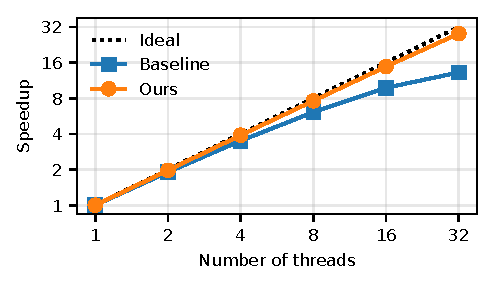
\includegraphics[width=\columnwidth]{speedup}
  \caption{Speedup on 1--32 threads (higher is better).}
  % \Description 是 ACM 要求的無障礙替代文字，不會印在 PDF 上
  \Description{Line chart of speedup versus thread count; Ours scales
    close to ideal while the baseline flattens after 8 threads.}
  \label{fig:speedup}
\end{figure}

\section{Related Work}
\label{sec:related}

\paragraph{Task-parallel runtimes.}
Cilk~\cite{blumofe1995cilk} introduced work stealing ...

\paragraph{Parallel programming models.}
OpenMP~\cite{dagum1998openmp} ... The textbook by
Herlihy et al.~\cite{herlihy2020art} ...

\section{Conclusion}
\label{sec:conclusion}

This paper presented \sys, ...


%% 致謝：投稿版會自動隱藏（anonymous）。
%% PPoPP 規定：若使用生成式 AI 協助撰寫文字、程式、圖表，須在此揭露。
\begin{acks}
This work was supported by ... (funding agency, grant number).
\end{acks}

\bibliography{references}

%% PPoPP 不允許 appendix，請勿在此加入 \appendix。
\end{document}
